\section{Тригонометрия решения}
1. $\cfrac{\cos(3\alpha)+\cos(4\alpha)+\cos(5\alpha)}{\sin(3\alpha)+\sin(4\alpha)+\sin(5\alpha)}=\cfrac{2\cos(4\alpha)\cos(\alpha)+\cos(4\alpha)}{2\sin(4\alpha)\cos(\alpha)+
\sin(4\alpha)}=\cfrac{\cos(4\alpha)(2\cos(\alpha)+1)}{\sin(4\alpha)(2\cos(\alpha)+1)}=ctg(4\alpha).$\\
2. $\cfrac{\cos(6\alpha)+\cos(8\alpha)+\cos(10\alpha)}{\sin(6\alpha)+\sin(8\alpha)+\sin(10\alpha)}=\cfrac{2\cos(8\alpha)\cos(2\alpha)+\cos(8\alpha)}{2\sin(8\alpha)\cos(2\alpha)+
\sin(8\alpha)}=\cfrac{\cos(8\alpha)(2\cos(2\alpha)+1)}{\sin(8\alpha)(2\cos(2\alpha)+1)}=ctg(8\alpha).$\\
3. Если $\alpha-\cfrac{\pi}{4}$ находится в $III$ четверти, то $\alpha+\cfrac{\pi}{4}$ находится в $IV$ четверти, его косинус положителен и равен $\cos\left(\alpha+\cfrac{\pi}{4}
ight)=\sqrt{1-\cfrac{144}{169}}=\cfrac{5}{13}.$ Тогда $\sin\left(2\alpha+\cfrac{\pi}{2}
ight)=2\left(-\cfrac{12}{13}
ight)\cdot
\cfrac{5}{13}=-\cfrac{120}{169}=\cos(2\alpha).$ Так как $\alpha+\cfrac{\pi}{4}$ находится в $IV$ четверти, его синус равен $-\cfrac{12}{13},$ это угол близкий
к $\cfrac{3\pi}{2},$ значит $\alpha$ находится в $III$ четверти, поэтому его косинус отрицателен и равен $\cos(\alpha)=-\sqrt{\cfrac{-\cfrac{120}{169}+1}{2}}=-\cfrac{7\sqrt{2}}{26}.$\\
4. Если $\alpha-\cfrac{\pi}{4}$ находится во $II$ четверти, то $\alpha-\cfrac{3\pi}{4}$ находится в $I$ четверти, его синус положителен и равен $\sin\left(\alpha-\cfrac{3\pi}{4}
ight)=\sqrt{1-\cfrac{25}{169}}=\cfrac{12}{13}.$ Тогда $\sin\left(2\alpha-\cfrac{3\pi}{2}
ight)=2\cdot\cfrac{12}{13}\cdot
\cfrac{5}{13}=\cfrac{120}{169}=\cos(2\alpha).$ Так как $\alpha-\cfrac{3\pi}{4}$ находится в $I$ четверти, его синус равен $\cfrac{12}{13},$ это угол близкий
к $\cfrac{\pi}{2},$ значит $\alpha$ находится в $III$ четверти, поэтому его синус отрицателен и равен $\sin(\alpha)=-\sqrt{\cfrac{1-\cfrac{120}{169}}{2}}=-\cfrac{7\sqrt{2}}{26}.$\\
5. $tg(2\alpha)=\cfrac{2tg(\alpha)}{1-tg^2(\alpha)}=\cfrac{1}{\sqrt{3}},\ 1-tg^2(\alpha)=2\sqrt{3}tg(\alpha),\ tg^2(\alpha)+2\sqrt{3}tg(\alpha)-1=0,\
tg(\alpha)=2-\sqrt{3}$ или $tg(\alpha)=-2-\sqrt{3}.$ В первом случае $\sin(\alpha)=(2-\sqrt{3})\cos(\alpha)$ и $(4-4\sqrt{3}+3)\cos^2(\alpha)+\cos^2(\alpha)=1,\
\cos^2(\alpha)=\cfrac{1}{4(2-\sqrt{3})}=\cfrac{4+2\sqrt{3}}{8},\ \cos(\alpha)=\pm\cfrac{\sqrt{3}+1}{2\sqrt{2}}.$ Тогда $\sin(\alpha)=\cfrac{2\sqrt{3}+2-3-\sqrt{3}}{2\sqrt{2}}=\cfrac{\sqrt{3}-1}{2\sqrt{2}}$ или $\sin(\alpha)=\cfrac{1-\sqrt{3}}{2\sqrt{2}}.$ Поэтому $\sin(\alpha)+\cos(\alpha)=\cfrac{\sqrt{3}-1}{2\sqrt{2}}+\cfrac{\sqrt{3}+1}{2\sqrt{2}}=\cfrac{\sqrt{6}}{2}$ или $\sin(\alpha)+\cos(\alpha)=\cfrac{1-\sqrt{3}}{2\sqrt{2}}+\cfrac{-1-\sqrt{3}}{2\sqrt{2}}=-\cfrac{\sqrt{6}}{2}.$ Во втором случае $\sin(\alpha)=(-2-\sqrt{3})\cos(\alpha)$ и $(4+4\sqrt{3}+3)\cos^2(\alpha)+\cos^2(\alpha)=1,\
\cos^2(\alpha)=\cfrac{1}{4(2+\sqrt{3})}=\cfrac{4-2\sqrt{3}}{8},\ \cos(\alpha)=\pm\cfrac{\sqrt{3}-1}{2\sqrt{2}}.$ Тогда $\sin(\alpha)=\cfrac{-2\sqrt{3}+2-3+\sqrt{3}}{2\sqrt{2}}=\cfrac{-\sqrt{3}-1}{2\sqrt{2}}$ или $\sin(\alpha)=\cfrac{\sqrt{3}+1}{2\sqrt{2}}.$ Поэтому $\sin(\alpha)+\cos(\alpha)=\cfrac{-\sqrt{3}-1}{2\sqrt{2}}+\cfrac{\sqrt{3}-1}{2\sqrt{2}}=-\cfrac{\sqrt{2}}{2}$ или $\sin(\alpha)+\cos(\alpha)=\cfrac{\sqrt{3}+1}{2\sqrt{2}}+\cfrac{1-\sqrt{3}}{2\sqrt{2}}=\cfrac{\sqrt{2}}{2}.$ Таким образом, $\sin(\alpha)+\cos(\alpha)\in\left\{\pm\cfrac{\sqrt{2}}{2};\pm\cfrac{\sqrt{6}}{2}
ight\}.$\\
6. $ctg(2\alpha)=\cfrac{ctg^2(\alpha)-1}{2ctg(\alpha)}=\sqrt{3},\ ctg^2(\alpha)-1=2\sqrt{3}ctg(\alpha),\ ctg^2(\alpha)-2\sqrt{3}ctg(\alpha)-1=0,\
ctg(\alpha)=2+\sqrt{3}$ или $ctg(\alpha)=-2+\sqrt{3}.$ В первом случае $\cos(\alpha)=(2+\sqrt{3})\sin(\alpha)$ и $(4+4\sqrt{3}+3)\sin^2(\alpha)+\sin^2(\alpha)=1,\
\sin^2(\alpha)=\cfrac{1}{4(2+\sqrt{3})}=\cfrac{4-2\sqrt{3}}{8},\ \sin(\alpha)=\pm\cfrac{\sqrt{3}-1}{2\sqrt{2}}.$ Тогда $\cos(\alpha)=\cfrac{2\sqrt{3}-2+3-\sqrt{3}}{2\sqrt{2}}=\cfrac{\sqrt{3}+1}{2\sqrt{2}}$ или $\cos(\alpha)=\cfrac{-1-\sqrt{3}}{2\sqrt{2}}.$ Поэтому $\sin(\alpha)-\cos(\alpha)=\cfrac{\sqrt{3}-1}{2\sqrt{2}}-\cfrac{\sqrt{3}+1}{2\sqrt{2}}=-\cfrac{\sqrt{2}}{2}$ или $\sin(\alpha)-\cos(\alpha)=\cfrac{1-\sqrt{3}}{2\sqrt{2}}-\cfrac{-1-\sqrt{3}}{2\sqrt{2}}=\cfrac{\sqrt{2}}{2}.$ Во втором случае $\cos(\alpha)=(-2+\sqrt{3})\sin(\alpha)$ и $(4-4\sqrt{3}+3)\sin^2(\alpha)+\sin^2(\alpha)=1,\
\sin^2(\alpha)=\cfrac{1}{4(2-\sqrt{3})}=\cfrac{4+2\sqrt{3}}{8},\ \sin(\alpha)=\pm\cfrac{\sqrt{3}+1}{2\sqrt{2}}.$ Тогда $\cos(\alpha)=\cfrac{-2\sqrt{3}-2+3+\sqrt{3}}{2\sqrt{2}}=\cfrac{1-\sqrt{3}}{2\sqrt{2}}$ или $\cos(\alpha)=\cfrac{\sqrt{3}-1}{2\sqrt{2}}.$ Поэтому $\sin(\alpha)-\cos(\alpha)=\cfrac{\sqrt{3}+1}{2\sqrt{2}}-\cfrac{1-\sqrt{3}}{2\sqrt{2}}=\cfrac{\sqrt{6}}{2}$ или $\sin(\alpha)-\cos(\alpha)=\cfrac{-\sqrt{3}-1}{2\sqrt{2}}-\cfrac{\sqrt{3}-1}{2\sqrt{2}}=-\cfrac{\sqrt{6}}{2}.$ Таким образом, $\sin(\alpha)-\cos(\alpha)\in\left\{\pm\cfrac{\sqrt{2}}{2};\pm\cfrac{\sqrt{6}}{2}
ight\}.$\\
7. $f(x)=-\sqrt{\sin^2\left(\cfrac{x}{2}
ight)}+\cfrac{\cos\left(\cfrac{x}{2}
ight)-\cos\left(\cfrac{3x}{2}
ight)}
{\sqrt{2-2\cos(2x)}}=-\left|\sin\left(\cfrac{x}{2}
ight)
ight|+\cfrac{-2\sin(x)\sin\left(-\cfrac{x}{2}
ight)}{\sqrt{4\sin^2(x)}}=
-\left|\sin\left(\cfrac{x}{2}
ight)
ight|+\cfrac{\sin(x)\sin\left(\cfrac{x}{2}
ight)}{|\sin(x)|}.$ Таким образом, при $x\in\left(-\pi;\pi
ight)+2\pi k\ (k\in \mathbb{Z})$ имеем $f(x)=0,$ а при $x\in\left(\pi;3\pi
ight)+2\pi k\ (k\in \mathbb{Z})$ имеем $f(x)=-2\sin\left(\cfrac{x}{2}
ight)$ за исключением точек $x=\pi k\ (k\in \mathbb{Z}),$ которые являются выколотыми.
$$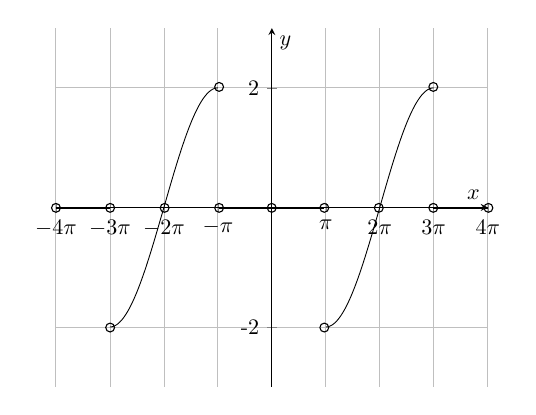
\begin{tikzpicture}[scale=0.8]
\tikzset{line02/.style={line width =0.8pt}}
\begin{axis}[
    axis lines = middle,
    grid=major,
    legend pos={south west},
    xlabel = {$x$},
    ylabel = {$y$},
    ymin=-3,
    ymax=3,
    xtick={-12.57,-9.42,-6.28,-3.14, 3.14, 6.28, 9.42, 12.57},
    xticklabels={$-4\pi$, $-3\pi$, $-2\pi$, $-\pi$, $\pi$, $2\pi$, $3\pi$, $4\pi$},
    ytick={2,-2},
    yticklabels={2,-2}          ]
	\addplot[domain=pi:3*pi, samples=100, color=black] {-2*sin(deg(x/2))};
    \addplot[domain=-3*pi:-pi, samples=100, color=black] {-2*sin(deg(x/2))};
    \addplot[domain=3*pi:4*pi, samples=100, color=black] {0};
    \addplot[domain=-4*pi:-3*pi, samples=100, color=black] {0};
%\addplot[domain=-3.1:2.5, samples=100, color=red] {70*abs(1-2*abs(abs(x)-2))-10*x^2+10*x-70};
	%\addlegendentry{$\text{Рис. 1}$};
\end{axis}
%\draw[line02] (0.9,2.84) -- (2.55,2.84);
%\draw[line02] (4.3,2.84) -- (5.95,2.84);
\draw[line02] (0,2.84) -- (0.86,2.84);
\draw[line02] (2.59,2.84) -- (4.26,2.84);
\draw[line02] (5.99,2.84) -- (6.865,2.84);
\draw (0.86,2.84) circle (2pt);
\draw (2.59,2.84) circle (2pt);
\draw (0.86,0.94) circle (2pt);
\draw (2.59,4.76) circle (2pt);
\draw (1.725,2.84) circle (2pt);
\draw (0,2.84) circle (2pt);

\draw (3.425,2.84) circle (2pt);

\draw (4.26,0.94) circle (2pt);
\draw (5.99,2.84) circle (2pt);
\draw (4.26,2.84) circle (2pt);
\draw (5.99,4.76) circle (2pt);
\draw (5.125,2.84) circle (2pt);

\draw (6.865,2.84) circle (2pt);
\end{tikzpicture}$$
8. $f(x)=\cfrac{\cos\left(\cfrac{3x}{2}
ight)-\cos\left(\cfrac{x}{2}
ight)}
{\sqrt{\cos^2(x)+\sin^2(x)-2\cos(2x)+1}}+\left|\sin\left(\cfrac{x}{2}
ight)
ight|=
\cfrac{-2\sin(x)\sin\left(\cfrac{x}{2}
ight)}{\sqrt{2(1-\cos(2x))}}+\left|\sin\left(\cfrac{x}{2}
ight)
ight|=$\\$
\cfrac{-2\sin(x)\sin\left(\cfrac{x}{2}
ight)}{\sqrt{4\sin^2(x)}}+\left|\sin\left(\cfrac{x}{2}
ight)
ight|=
\cfrac{-\sin(x)\sin\left(\cfrac{x}{2}
ight)}{|\sin(x)|}+\left|\sin\left(\cfrac{x}{2}
ight)
ight|.$
Таким образом, при $x\in\left(-\pi;\pi
ight)+2\pi k\ (k\in \mathbb{Z})$ имеем $f(x)=0,$ а при $x\in\left(\pi;3\pi
ight)+2\pi k\ (k\in \mathbb{Z})$ имеем $f(x)=2\sin\left(\cfrac{x}{2}
ight)$ за исключением точек $x=\pi k\ (k\in \mathbb{Z}),$ которые являются выколотыми.
$$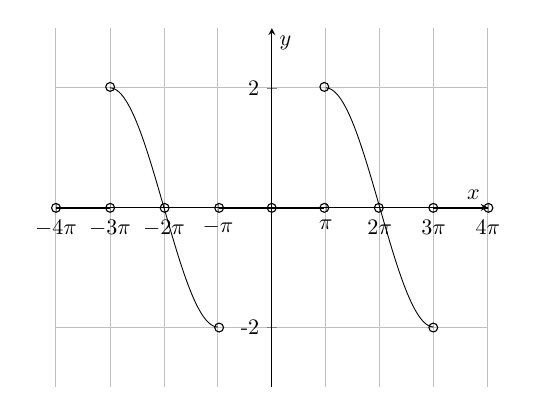
\begin{tikzpicture}[scale=0.8]
\tikzset{line02/.style={line width =0.8pt}}
\begin{axis}[
    axis lines = middle,
    grid=major,
    legend pos={south west},
    xlabel = {$x$},
    ylabel = {$y$},
    ymin=-3,
    ymax=3,
    xtick={-12.57,-9.42,-6.28,-3.14, 3.14, 6.28, 9.42, 12.57},
    xticklabels={$-4\pi$, $-3\pi$, $-2\pi$, $-\pi$, $\pi$, $2\pi$, $3\pi$, $4\pi$},
    ytick={2,-2},
    yticklabels={2,-2}          ]
	\addplot[domain=pi:3*pi, samples=100, color=black] {2*sin(deg(x/2))};
    \addplot[domain=-3*pi:-pi, samples=100, color=black] {2*sin(deg(x/2))};
    \addplot[domain=3*pi:4*pi, samples=100, color=black] {0};
    \addplot[domain=-4*pi:-3*pi, samples=100, color=black] {0};
%\addplot[domain=-3.1:2.5, samples=100, color=red] {70*abs(1-2*abs(abs(x)-2))-10*x^2+10*x-70};
	%\addlegendentry{$\text{Рис. 1}$};
\end{axis}
%\draw[line02] (0.9,2.84) -- (2.55,2.84);
%\draw[line02] (4.3,2.84) -- (5.95,2.84);
\draw[line02] (0,2.84) -- (0.86,2.84);
\draw[line02] (2.59,2.84) -- (4.26,2.84);
\draw[line02] (5.99,2.84) -- (6.865,2.84);
\draw (0.86,2.84) circle (2pt);
\draw (2.59,2.84) circle (2pt);
\draw (0.86,4.76) circle (2pt);
\draw (2.59,0.94) circle (2pt);
\draw (1.725,2.84) circle (2pt);
\draw (0,2.84) circle (2pt);

\draw (3.425,2.84) circle (2pt);

\draw (4.26,4.76) circle (2pt);
\draw (5.99,2.84) circle (2pt);
\draw (4.26,2.84) circle (2pt);
\draw (5.99,0.94) circle (2pt);
\draw (5.125,2.84) circle (2pt);

\draw (6.865,2.84) circle (2pt);
\end{tikzpicture}$$
9. $\cfrac{1-\cos(2\alpha)+\sin(2\alpha)}{1+\cos(2\alpha)+\sin(2\alpha)}=
\cfrac{2\sin^2(\alpha)+2\sin(\alpha)\cos(\alpha)}{2\cos^2(\alpha)+2\sin(\alpha)\cos(\alpha)}=
\cfrac{2\sin(\alpha)(\sin(\alpha)+\cos(\alpha))}{2\cos(\alpha)(\sin(\alpha)+\cos(\alpha))}=tg(\alpha).$\\
10. $\cfrac{1+\cos(\alpha)+\cos(2\alpha)+\cos(3\alpha)}{\cos(\alpha)+\cos(2\alpha)}=
\cfrac{1+\cos(\alpha)+2\cos^2(\alpha)-1+4\cos^3(\alpha)-3\cos(\alpha)}{\cos(\alpha)+2\cos^2(\alpha)-1}=$\\$
\cfrac{\cos(\alpha)(4\cos^2(\alpha)+2\cos(\alpha)-2)}{2\cos^2(\alpha)+\cos(\alpha)-1}=2\cos(\alpha).$\\
11. Так как $\sin (90^\circ-\alpha)=\cos \alpha,$ а $\cos (90^\circ-\alpha)=\sin \alpha,$ получим $tg(\alpha)\cdot tg(90^\circ-\alpha)=1.$ Таким образом,
$tg(41^\circ)\cdot tg(42^\circ)\cdot \ldots \cdot tg(48^\circ)\cdot tg(49^\circ)=tg(41^\circ)\cdot tg(49^\circ)\cdot
tg(42^\circ)\cdot tg(48^\circ)\cdot
tg(43^\circ)\cdot tg(47^\circ)\cdot
tg(44^\circ)\cdot tg(46^\circ)\cdot tg(45^\circ)=1.$\\
12. Так как $\sin (90^\circ-\alpha)=\cos \alpha,$ а $\cos (90^\circ-\alpha)=\sin \alpha,$ получим $ctg(\alpha)\cdot ctg(90^\circ-\alpha)=1.$ Таким образом,
$ctg(41^\circ)\cdot ctg(42^\circ)\cdot \ldots \cdot ctg(48^\circ)\cdot ctg(49^\circ)=ctg(41^\circ)\cdot ctg(49^\circ)\cdot
ctg(42^\circ)\cdot ctg(48^\circ)\cdot
ctg(43^\circ)\cdot ctg(47^\circ)\cdot
ctg(44^\circ)\cdot ctg(46^\circ)\cdot ctg(45^\circ)=1.$\\
13. $\cfrac{\sin(\alpha)}{1+\cos(\alpha)}+ctg(\alpha)=\cfrac{\sin(\alpha)}{1+\cos(\alpha)}+\cfrac{\cos(\alpha)}{\sin(\alpha)}=\cfrac{\sin^2(\alpha)+\cos(\alpha)+\cos^2(\alpha)}{(1+\cos(\alpha))\sin(\alpha)}
=\cfrac{1+\cos(\alpha)}{(1+\cos(\alpha))\sin(\alpha)}=\cfrac{1}{\sin(\alpha)}.$\\
14. $\cfrac{\cos(\alpha)}{1+\sin(\alpha)}+tg(\alpha)=\cfrac{\cos(\alpha)}{1+\sin(\alpha)}+\cfrac{\sin(\alpha)}{\cos(\alpha)}=
\cfrac{\cos^2(\alpha)+\sin(\alpha)+\sin^2(\alpha)}{(1+\sin(\alpha))\cos(\alpha)}=\cfrac{1+\sin(\alpha)}{(1+\sin(\alpha))\cos(\alpha)}=\cfrac{1}{\cos(\alpha)}.$\\
15. Так как $\sin (180^\circ-\alpha)=\sin \alpha$ и $\cos (180^\circ-\alpha)=- \cos \alpha,$ имеем $tg(180^\circ-\alpha)=-tg(\alpha).$ Тогда $ctg(160^\circ)\cdot tg(20^\circ)\cdot ctg(135^\circ)=\cfrac{tg(20^\circ)}{-tg(20^\circ)}\cdot(-1)=1.$\\
16. Так как $\sin (180^\circ-\alpha)=\sin \alpha$ и $\cos (180^\circ-\alpha)=- \cos \alpha,$ имеем $tg(180^\circ-\alpha)=-tg(\alpha).$ Тогда $ctg(140^\circ)\cdot tg(40^\circ)\cdot tg(135^\circ)=\cfrac{tg(40^\circ)}{-tg(40^\circ)}\cdot(-1)=1.$\\
17. Если  $90^\circ<\alpha<180^\circ,$ то $\sin(\alpha)>0.$ Тогда $\sin(\alpha)=\sqrt{1-\cfrac{25}{169}}=\cfrac{12}{13}$ и $tg(\alpha)=\cfrac{\cfrac{12}{13}}{-\cfrac{5}{13}}=-\cfrac{12}{5}.$\\
18. Если  $90^\circ<\alpha<180^\circ,$ то $\cos(\alpha)<0.$ Тогда $\cos(\alpha)=-\sqrt{1-\cfrac{25}{169}}=-\cfrac{12}{13}$ и $ctg(\alpha)=\cfrac{-\cfrac{12}{13}}{\cfrac{5}{13}}=-\cfrac{12}{5}.$\\
19. Если $\alpha-\cfrac{\pi}{3}$ находится в III четверти, то $\alpha-\cfrac{\pi}{3}+\cfrac{\pi}{2}=\alpha+\cfrac{\pi}{6}$ находится в IV четверти и $\cos\left(\alpha+\cfrac{\pi}{6}
ight)=\sqrt{1-\cfrac{169}{196}}=\cfrac{3\sqrt{3}}{14}.$ Тогда $\cos(\alpha)=\cos\left(\alpha+\cfrac{\pi}{6}-\cfrac{\pi}{6}
ight)=
\cfrac{3\sqrt{3}}{14}\cdot\cfrac{\sqrt{3}}{2}-\cfrac{13}{14}\cdot\cfrac{1}{2}=-\cfrac{1}{7}.$\\
20. Если $\alpha-\cfrac{\pi}{4}$ находится в I четверти, то $\alpha-\cfrac{\pi}{4}-\cfrac{\pi}{2}=\alpha-\cfrac{3\pi}{4}$ находится в IV четверти и $\sin\left(\alpha-\cfrac{3\pi}{4}
ight)=-\sqrt{1-\cfrac{25}{169}}=-\cfrac{12}{13}.$ Тогда $\sin(\alpha)=\sin\left(\alpha-\cfrac{3\pi}{4}+\cfrac{3\pi}{4}
ight)=
-\cfrac{12}{13}\cdot\left(-\cfrac{\sqrt{2}}{2}
ight)-\cfrac{5}{13}\cdot\cfrac{\sqrt{2}}{2}=\cfrac{7\sqrt{2}}{26}.$\\
21. Если $\cfrac{\pi}{2}<\alpha<\pi,$ то  $\cos(\alpha)=-\sqrt{1-\cfrac{49}{625}}=-\cfrac{24}{25}.$ Тогда $\sin(2\alpha)=2\cdot\cfrac{7}{25}\cdot\left(-\cfrac{24}{25}
ight)=-\cfrac{336}{625}.$\\
22. Если $-\cfrac{\pi}{2}<\alpha<0,$ то  $\sin(\alpha)=-\sqrt{1-\cfrac{25}{169}}=-\cfrac{12}{13}.$ Тогда $\sin(2\alpha)=2\cdot\left(-\cfrac{12}{13}
ight)\cdot\cfrac{5}{13}=-\cfrac{120}{169}.$\\
23. Если $\pi<\alpha<\cfrac{3\pi}{2},$ то  $\cos(\alpha)=-\sqrt{1-\cfrac{49}{625}}=-\cfrac{24}{25}.$ Тогда $\sin(2\alpha)=2\cdot\left(-\cfrac{7}{25}
ight)\cdot\left(-\cfrac{24}{25}
ight)=\cfrac{336}{625}.$\\
24. Если $\pi<\alpha<\cfrac{3\pi}{2},$ то  $\sin(\alpha)=-\sqrt{1-\cfrac{25}{169}}=-\cfrac{12}{13}.$ Тогда $\sin(2\alpha)=2\cdot\left(-\cfrac{12}{13}
ight)\cdot\left(-\cfrac{5}{13}
ight)=\cfrac{120}{169}.$\\
25. $\cos(2\alpha)=1-2\cdot\cfrac{144}{169}=-\cfrac{119}{169}.$\\
26. Если $\cfrac{\pi}{2}<\alpha<\pi,$ то  $\sin(\alpha)=\sqrt{1-\cfrac{25}{169}}=\cfrac{12}{13}.$ Тогда $\sin(2\alpha)=2\cdot\cfrac{12}{13}\cdot\left(-\cfrac{5}{13}
ight)=-\cfrac{120}{169}.$\\
27. В прямоугольном треугольнике два непрямых угла являются острыми, поэтому\\ $\cos(A)=\sqrt{1-\cfrac{49}{625}}=\cfrac{24}{25}.$\\
28. В прямоугольном треугольнике два непрямых угла являются острыми, поэтому\\ $\cos(A)=\sqrt{1-\cfrac{576}{625}}=\cfrac{7}{25}.$\\
29. Если $tg(\alpha)=3,$ то $\cfrac{\sin(\alpha)}{\cos(\alpha)}=3,\ \sin(\alpha)=3\cos(\alpha).$ По основному тригонометрическому тождеству имеем соотношение
$\sin^2(\alpha)+\cos^2(\alpha)=9\cos^2(\alpha)+\cos^2(\alpha)=10\cos^2(\alpha)=1,$ откуда $\cos^2(\alpha)=\cfrac{1}{10}.$ По формуле синуса двойного угла получаем
равенство $\sin(2\alpha)=2\sin(\alpha)\cos(\alpha)=2\cfrac{\sin(\alpha)}{\cos(\alpha)}\cdot\cos^2(\alpha)=2\cdot3\cdot\cfrac{1}{10}=\cfrac{3}{5}.$\\
30. Если $ctg(\alpha)=0,5,$ то $\cfrac{\cos(\alpha)}{\sin(\alpha)}=0,5,\ \sin(\alpha)=2\cos(\alpha).$ По основному тригонометрическому тождеству имеем соотношение
$\sin^2(\alpha)+\cos^2(\alpha)=4\cos^2(\alpha)+\cos^2(\alpha)=5\cos^2(\alpha)=1,$ откуда $\cos^2(\alpha)=\cfrac{1}{5}.$ По формуле косинуса двойного угла получаем
равенство $\cos(2\alpha)=2\cos^2(\alpha)-1=\cfrac{2}{5}-1=-\cfrac{3}{5}.$\\
31. $\cfrac{\sin(\alpha)+2\cos(\alpha)}{\sin(\alpha)-\cos(\alpha)}=\cfrac{\cfrac{\sin(\alpha)}{\cos(\alpha)}+2}{\cfrac{\sin(\alpha)}{\cos(\alpha)}-1}=
\cfrac{tg(\alpha)+2}{tg(\alpha)-1}=\cfrac{\cfrac{5}{4}+2}{\cfrac{5}{4}-1}=13.$

ewpage
